% Edgeworth box - Optimal allocation of inputs for two economies
% Author: Thomas de Graaff
\documentclass[border=10pt]{standalone} 
%%%<
\usepackage{verbatim}
%%%>
\usepackage{pgfplots}
\pgfplotsset{width=7cm, compat=1.10}
\usetikzlibrary{calc, intersections}	       %allows coordinate calculations.
\begin{comment}
:Title: Edgeworth box - Optimal allocation of inputs for two economies
:Tags: 2D, Economics
:Author: Thomas de Graafif
:Slug: edgeworth-box

This edgeworth box describes the optimal allocation (pareto efficient) of
inputs for the Cobb-Douglas production functions of two countries/regions
(A and B). In addition, it shows the initial endowments of inputs and the
resulting area of patero improvements. Parameters that can be changes:
capital intensity parameter region A/B, total amount of labour and capital
in A and B, and initial endowment K and L in A.
\end{comment}
\begin{document}   
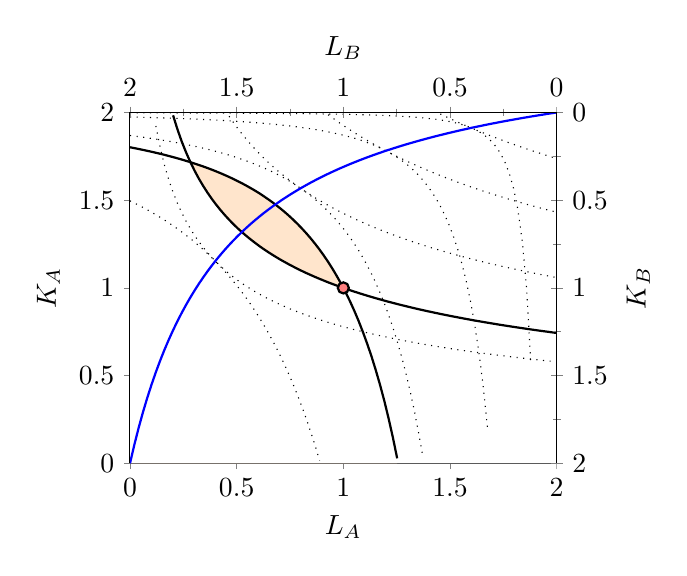
\begin{tikzpicture}[scale=1,thick]
  % Define parameters
  \def\alpha{0.7}  % Capital intensity parameter for region A.
  \def\beta{0.3}   % Capital intensity parameter for region B.
  \def\L{2}        % Total amount of labour in economy.
  \def\K{2}        % Total amount of capital in economy.
  \def\PK{0.5}     % Percentage K in A in initial endowment.
  \def\PL{0.5}     % Percentage L in A in initial endowment.

  % Define isoquants
  \def\InitYA{((\PL*\L)^(1-\alpha))*((\PK*\K)^(\alpha))}		
  \def\InitYB{(((1-\PL)*\L)^(1-\beta))*(((1-\PK)*\K)^(\beta))}

  \def\La{0.2*\L}
  \def\Lb{0.4*\L}
  \def\Lc{0.6*\L}
  \def\Ld{0.8*\L}

  \def\Ka{%
    \alpha*(1-\beta)*\K*\La/((1-\alpha)*\beta*(\L-\La)+\alpha*(1-\beta)*\La)}
  \def\Kb{%
    \alpha*(1-\beta)*\K*\Lb/((1-\alpha)*\beta*(\L-\Lb)+\alpha*(1-\beta)*\Lb)}
  \def\Kc{%
    \alpha*(1-\beta)*\K*\Lc/((1-\alpha)*\beta*(\L-\Lc)+\alpha*(1-\beta)*\Lc)}
  \def\Kd{%
    \alpha*(1-\beta)*\K*\Ld/((1-\alpha)*\beta*(\L-\Ld)+\alpha*(1-\beta)*\Ld)}

  \def\YAa{((\La)^(1-\alpha)*((\Ka)^\alpha)}
  \def\YAb{((\Lb)^(1-\alpha)*((\Kb)^\alpha)}
  \def\YAc{((\Lc)^(1-\alpha)*((\Kc)^\alpha)}
  \def\YAd{((\Ld)^(1-\alpha)*((\Kd)^\alpha)}

  \def\YBa{((\L-\La)^(1-\beta)*((\K-\Ka)^\beta)}
  \def\YBb{((\L-\Lb)^(1-\beta)*((\K-\Kb)^\beta)}
  \def\YBc{((\L-\Lc)^(1-\beta)*((\K-\Kc)^\beta)}
  \def\YBd{((\L-\Ld)^(1-\beta)*((\K-\Kd)^\beta)}

  \begin{axis}[
      restrict y to domain=0:\K,
      samples = 100,     		
      xmin = 0, xmax = \L,
      ymin = 0, ymax = \K,
      xlabel = $L_A$,
      ylabel = $K_A$,
      axis y line = left,    
      axis x line = bottom,
      y axis line style = {-}, 
      x axis line style = {-}
    ]
    \def\LineA{(\InitYA/\x^(1-\alpha))^(1/\alpha))};
    \def\LineB {\K-(\InitYB/(\L-\x)^(1-\beta))^(1/\beta)};
			
    % color the area with all pareto improvements			
    \addplot [fill=orange!40, opacity=0.5, draw=none,domain=0:\L] {\LineB}
      \closedcycle;
    \addplot [fill=white, draw=none,domain=0:\L] {\LineA} |- (axis cs:0,0)
      -- (axis cs:0,\K)--cycle; 

    %Draw isoquants
    \addplot[thin, dotted, mark=none, domain=0:\L]
      {(\YAa/\x^(1-\alpha))^(1/\alpha)};
    \addplot[thin, dotted, mark=none, domain=0:\L]
      {(\YAb/\x^(1-\alpha))^(1/\alpha)};
    \addplot[thick, mark=none, domain=0:\L] {(\LineA};
    \addplot[thin, dotted, mark=none, domain=0:\L]
      {(\YAc/\x^(1-\alpha))^(1/\alpha)};
    \addplot[thin, dotted, mark=none, domain=0:\L]
      {(\YAd/\x^(1-\alpha))^(1/\alpha)};

    \addplot[thin, dotted, mark=none, domain=0:\L]
      {\K-(\YBa/(\L-\x)^(1-\beta))^(1/\beta)};
    \addplot[thin, dotted, mark=none, domain=0:\L]
      {\K-(\YBb/(\L-\x)^(1-\beta))^(1/\beta)};
    \addplot[thick, mark=none, domain=0:\L] {\LineB};
    \addplot[thin, dotted, mark=none, domain=0:\L]
      {\K-(\YBc/(\L-\x)^(1-\beta))^(1/\beta)};
    \addplot[thin, dotted, mark=none, domain=0:\L]
      {\K-(\YBd/(\L-\x)^(1-\beta))^(1/\beta)};   
      
    % Draw contractcurve
    \addplot[mark=none, domain=0:\L, color=blue,thick]
      {\alpha*(1-\beta)*\K*\x/((1-\alpha)*\beta*(\L-\x)+\alpha*(1-\beta)*\x)};
    % Draw initial endowments
    \addplot[thick, mark=*, fill=red!50] coordinates {(\L*\PL,\K*\PK)};    
  \end{axis}

  % Draw mirrored axis
  \begin{axis}[
      restrict y to domain = 0:\K,
      minor tick num = 1,
      xlabel = $L_B$,
      ylabel = $K_B$,
      xmin = 0, xmax = \L,
      ymin = 0, ymax = \K,
      axis y line = right,
      axis x line = top,
      x dir = reverse,
      y dir = reverse,
      y axis line style = {-},
      x axis line style = {-}
    ]
  \end{axis}  
\end{tikzpicture}
\end{document} 
